\chapter{Pytropos (Analysis Implementation)}%
\label{pytropos-analysis-implementation}

Pytropos\footnote{There is an old trend where programs, companies and
  anything that could be named was named after some mythological
  creature from an ancient civilization. Thus, why could not this work
  also have a proper ancient-based name. Pytropos comes from the merge
  of Python and Atropos. In Greek mythology, Atropos was one of the
  three goddesses of fate who decided on the lives of humans, she was
  the goddess of death and the one who cut the thread of life.}\footnote{
  Homepage: \url{https://github.com/helq/pytropos}
}
is the Abstract Interpreter implemented in this work. The interpreter follows the rules
exposed in the previous chapter.

We explore how is Pytropos built, a brief history and some internal details.

% This chapter is divided into two parts. In the first part, we explore how is Pytropos
% built, a brief history and some internal details. The second part is a small guide on how
% to interpret Pytropos output over a couple of different examples.

\section{The big picture}\label{the-big-picture}

\begin{figure}
\begin{center}
  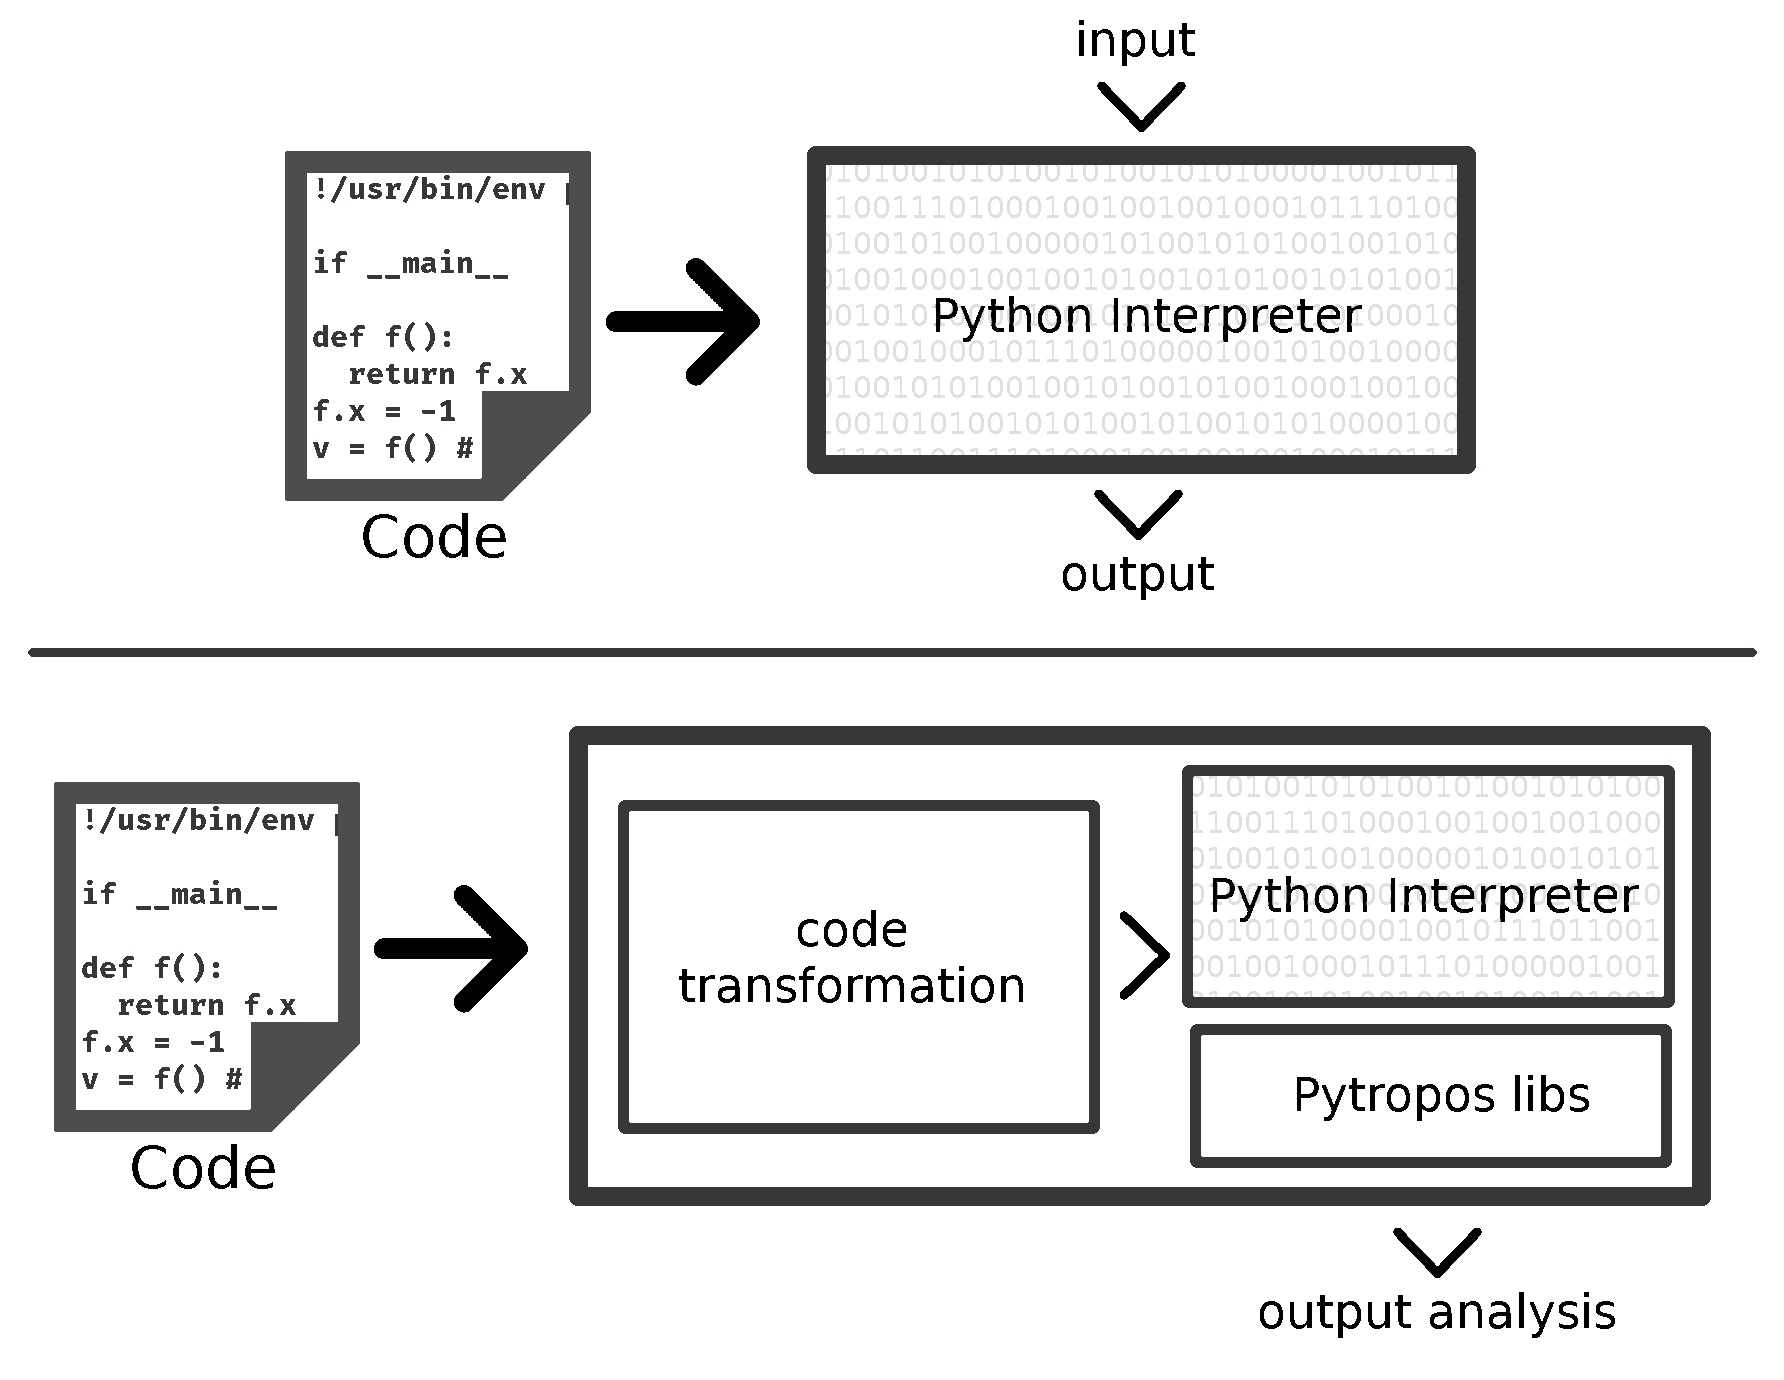
\includegraphics[width=0.6\textwidth]{figures/pytroposimage.png}
\end{center}
\caption{Up: black box step by step of executing a piece of code in Python (CPython). Down:
  Pytropos extension of Python. Pytropos transforms the code prior to run it by CPython.
  The transformation wraps the code to be run with the help of a custom library.
  \label{pytroposinter}}
\end{figure}

Pytropos works in a similar way as any other Python interpreter does. Pytropos reads code
and executes it sentence by sentence. Its main difference to CPython is that it does not
transform code into bytecode but it wraps the code before it is transformed into CPython
bytecode. The code is wrapped to use a library that implements the semantics of the
Abstract Interpreter. See Figure~\ref{pytroposinter}.

Similar to how Python works, Pytropos not only \enquote{runs} individual files but also
offers a REPL (Read-eval-print loop) to check small portions of code.

\section{Wrapped code + libs + interpreter vs.~from scratch interpreter}%
\label{wrapped-code-libs-interpreter-vs.from-scratch-interpreter}

The traditional methodology to build an interpreter is to code the parser and the
semantics of the language in one big program. For a language like Python, building an
interpreter from scratch would require considerable effort given the large amount of
characteristics Python comes with. A \enquote{complete} Python implementation would
require to implement--among other things--memory management, garbage collection, function
calling and return, dynamic type analysis, exception handling.

\textcite{ortin_towards_2015} showed how to build a Static Type Analysis by means of
rewriting the code to operate with the types of values rather than with the values
themselves, i.e.~the result of executing the code is not some values but some types. For
example, consider the following small piece of code:

\begin{pythoncode}
a = 2 + 4
b = a + "yep"  # this will fail
c = a / 2
\end{pythoncode}

Notice how even though the piece of code fails to run successfully,
we can determine the types of all variables. \pycode|a| has type
\pycode|int|, \pycode|b| has no type as it cannot be
computed, and \pycode|c| has type \pycode|float| because the
division of \pycode|int|s in Python 3 gives us back a \pycode|float|.

We can build a library that operates on types (rather than values) and
then we can rewrite the piece of code above into:

\begin{pythoncode}
import typeops as to
a = to.add(int, int)
b = to.add(a, str)
c = to.div(a, int)
\end{pythoncode}

If the library has properly defined the methods \pycode|add| and
\pycode|div|, we can be sure that the code will run without any error.
Notice that the library is able to find type mismatches by embedding
checks in the functions \pycode|add| and \pycode|div|. The library can,
effectively, perform Static Type Analysis on a piece of code.

Pytropos is implemented following the same strategy: a library that
operates over abstract values, and a transformation procedure that takes
the code and wraps it to use the library. The final step is to run the
wrapped code and collect the generated errors\footnote{%
  This strategy has been applied in the past for similar purposes, mainly to reuse
  infrastructure. It was used by \textcite{lauko_symbolic_2018} for symbolic computation
  of LLVM bytecode.
  %\inlinetodo{actually I'm not aware of any other example where this has been done :S}
  }.

The main advantage of translating code into wrapped code is the reuse of
infrastructure. One does not need to write all the infrastructure that
an interpreter needs. Pytropos does not implement its own call system,
heap management or garbage collection. All of it is managed by the
underlying Python implementation where the code is executed.

Nevertheless, this approach has three main disadvantages. First, all operations, function
calls, attribute access, subscript access and the whole Python semantics, must be coded
into the library and in the transformation function. Second, the place where any operation
has occurred must be preserved too, otherwise, it is impossible to find where an error has
occurred. Finally, all variable accesses must also be wrapped, otherwise the execution
would stop if one finds an undefined variable.  Because of all of this wrapping, the
transformation does not produce a simple, human-readable output.

To show, how currently Pytropos wraps and transforms the code consider the code below
from the piece of code above:

\begin{pythoncode}
import pytropos.internals as pt
st = pt.Store()
pt.loadBuiltinFuncs(st)
fn = 'test.py'
st[('a', ((1, 0), fn))] = pt.int(2).add(pt.int(4), pos=((1, 4), fn))
st[('b', ((2, 0), fn))] = st[('a', ((2, 4), fn))].add(pt.str('yep'), pos=((2, 4), fn))
st[('c', ((3, 0), fn))] = st[('a', ((3, 4), fn))].truediv(pt.int(2), pos=((3, 4), fn))
\end{pythoncode}

Not as nice as the first example.

Pytropos started out from the same idea as \textcite{ortin_towards_2015}
but it differs on its principal goal. Pytropos goal was not to perform
Static Type Analysis but Static Value Analysis. After working for three
months on a prototype, it became blatantly clear that trying to wrap the
code naïvely did not work very well, i.e.~the code was a hacky and not
very resilient. The library and transformation needed to be based on a
solid theoretical framework.

Enter Abstract Interpretation. Abstract Interpretation offers the ideal
framework for Static Value Analysis, it is well understood, with solid
theory and extensive work on it has been done for the last four decades.

\textcite{ortin_towards_2015} strategy alone may still be a good idea
for Static Type Analysis, but it may not work without a framework to
glue together the semantics of the language with those of the analysis.
Their legacy to Pytropos is the reuse of Python infrastructure by
wrapping the code and not building an interpreter from scratch.

\section{Assumptions}\label{assumptions}

Pytropos is limited to work only with Python 3.6 or higher. Pytropos
uses variable annotations to allow the user to specify the shape of
NumPy arrays when Pytropos is not able to \enquote{infer} their value.
Variable annotations were introduced on Python 3.6 \autocite{pep526}.

The goal of Pytropos is to warn the user when an operation will fail at runtime. It is not
a goal of Pytropos to verify the code and prove its correctness (Pytropos is not a tool
for verification).

Pytropos goal is not to replace MyPy, flake8, or any other static
analysis Python tool\footnote{I use MyPy and flake8 in every project and
  I am thankful for the years of effort put into these amazing tools.
  Thank you, guys!}. Pytropos is meant to be an aid for developers when
working with tensors.

Based on that, I present the main assumptions taken into account at the design stage of
Pytropos:

\begin{itemize}
\tightlist
\item The user wants as little warnings on the code as possible. Pytropos should warn the
  user for errors it is sure will occur at runtime.
\item The user cares only about the shape of tensors and not about their actual content.
\item If Pytropos is not able to infer the value of a variable, the user can (optionally)
  annotate the type/value of the variable. If the annotation is not more precise than the
  value that Pytropos has already inferred the inferred value will not be changed.
\end{itemize}

\section{Details about the guts}

To start with, I do not follow the structure defined in the previous chapter for how
elements are saved in memory. I did not explicitly defined a Heap (\(\Hea^\sharp\)) but
rather, I make use of Python's heap. The main reason to not define a custom Heap is the
cost associated to it, especially the definition of a Garbage Collector. The classes
\pycode|AbstractMutVal| and \pycode|Store|, the implementations of
\(\mathbf{Object}^\sharp\) and \(\Glo^\sharp\), respectively, do not point to
\(\mathbf{Addr}^\sharp\)s but they point to \pycode|PythonValue|s directly (again, because
CPython manages the heap not Pytropos). The global scope, \pycode|Store|, is an object
that takes a \pycode|str| and returns a \pycode|PythonValue|. An
\(\mathbf{Object}^\sharp\), \pycode|AbstractMutVal|, is an object that has an associated
type and operations, and it can point to any \pycode|PythonValue|.
%In this way, the Pytropos resembles more the graph representation than
%the classical Heap representation\footnote{Both representations are
%  explained in detail in the previous chapter}.

The class \pycode|PythonValue| implements the \(\mathbf{Val}^\sharp\) Abstract Domain. A
\pycode|PythonValue| is a wrapper around either an \pycode|AbstractValue| or an
\pycode|AbstractMutVal| (the implementations of \(\mathbf{PrimVal}^\sharp\) and
\(\mathbf{Object}^\sharp\)). Note that \pycode|AbstractMutVal| subclasses
\pycode|AbstractValue|, as well as do \pycode|Int|, \pycode|Float|, \pycode|NoneType| and
\pycode|Bool| which implement \(\text{Int}^\sharp\), \(\text{Float}^\sharp\),
\(\text{None}^\sharp\) and \(\text{Bool}^\sharp\), respectively.

\pycode|AbstractValue| is an abstract class that defines all the
operations supported (\pycode|+|, \pycode|*|, \ldots{}) by Pytropos, and
what it is required for a function call, subscript access and attribute
access. \pycode|AbstractValue|, in its turn, subclasses
\pycode|AbstractDomain| an abstract class that defines the methods every
Abstract Domain should have, namely \pycode|is_top()|, \pycode|join()|,
\pycode|top()| and \pycode|widen_op()|. \pycode|PythonValue| and
\pycode|Store|, unsurprisingly, also subclass \pycode|AbstractDomain|.

Figure~\ref{classPytropos} presents the class diagram showing the relationships
between the different components in Pytropos.

\begin{figure}
\begin{center}
  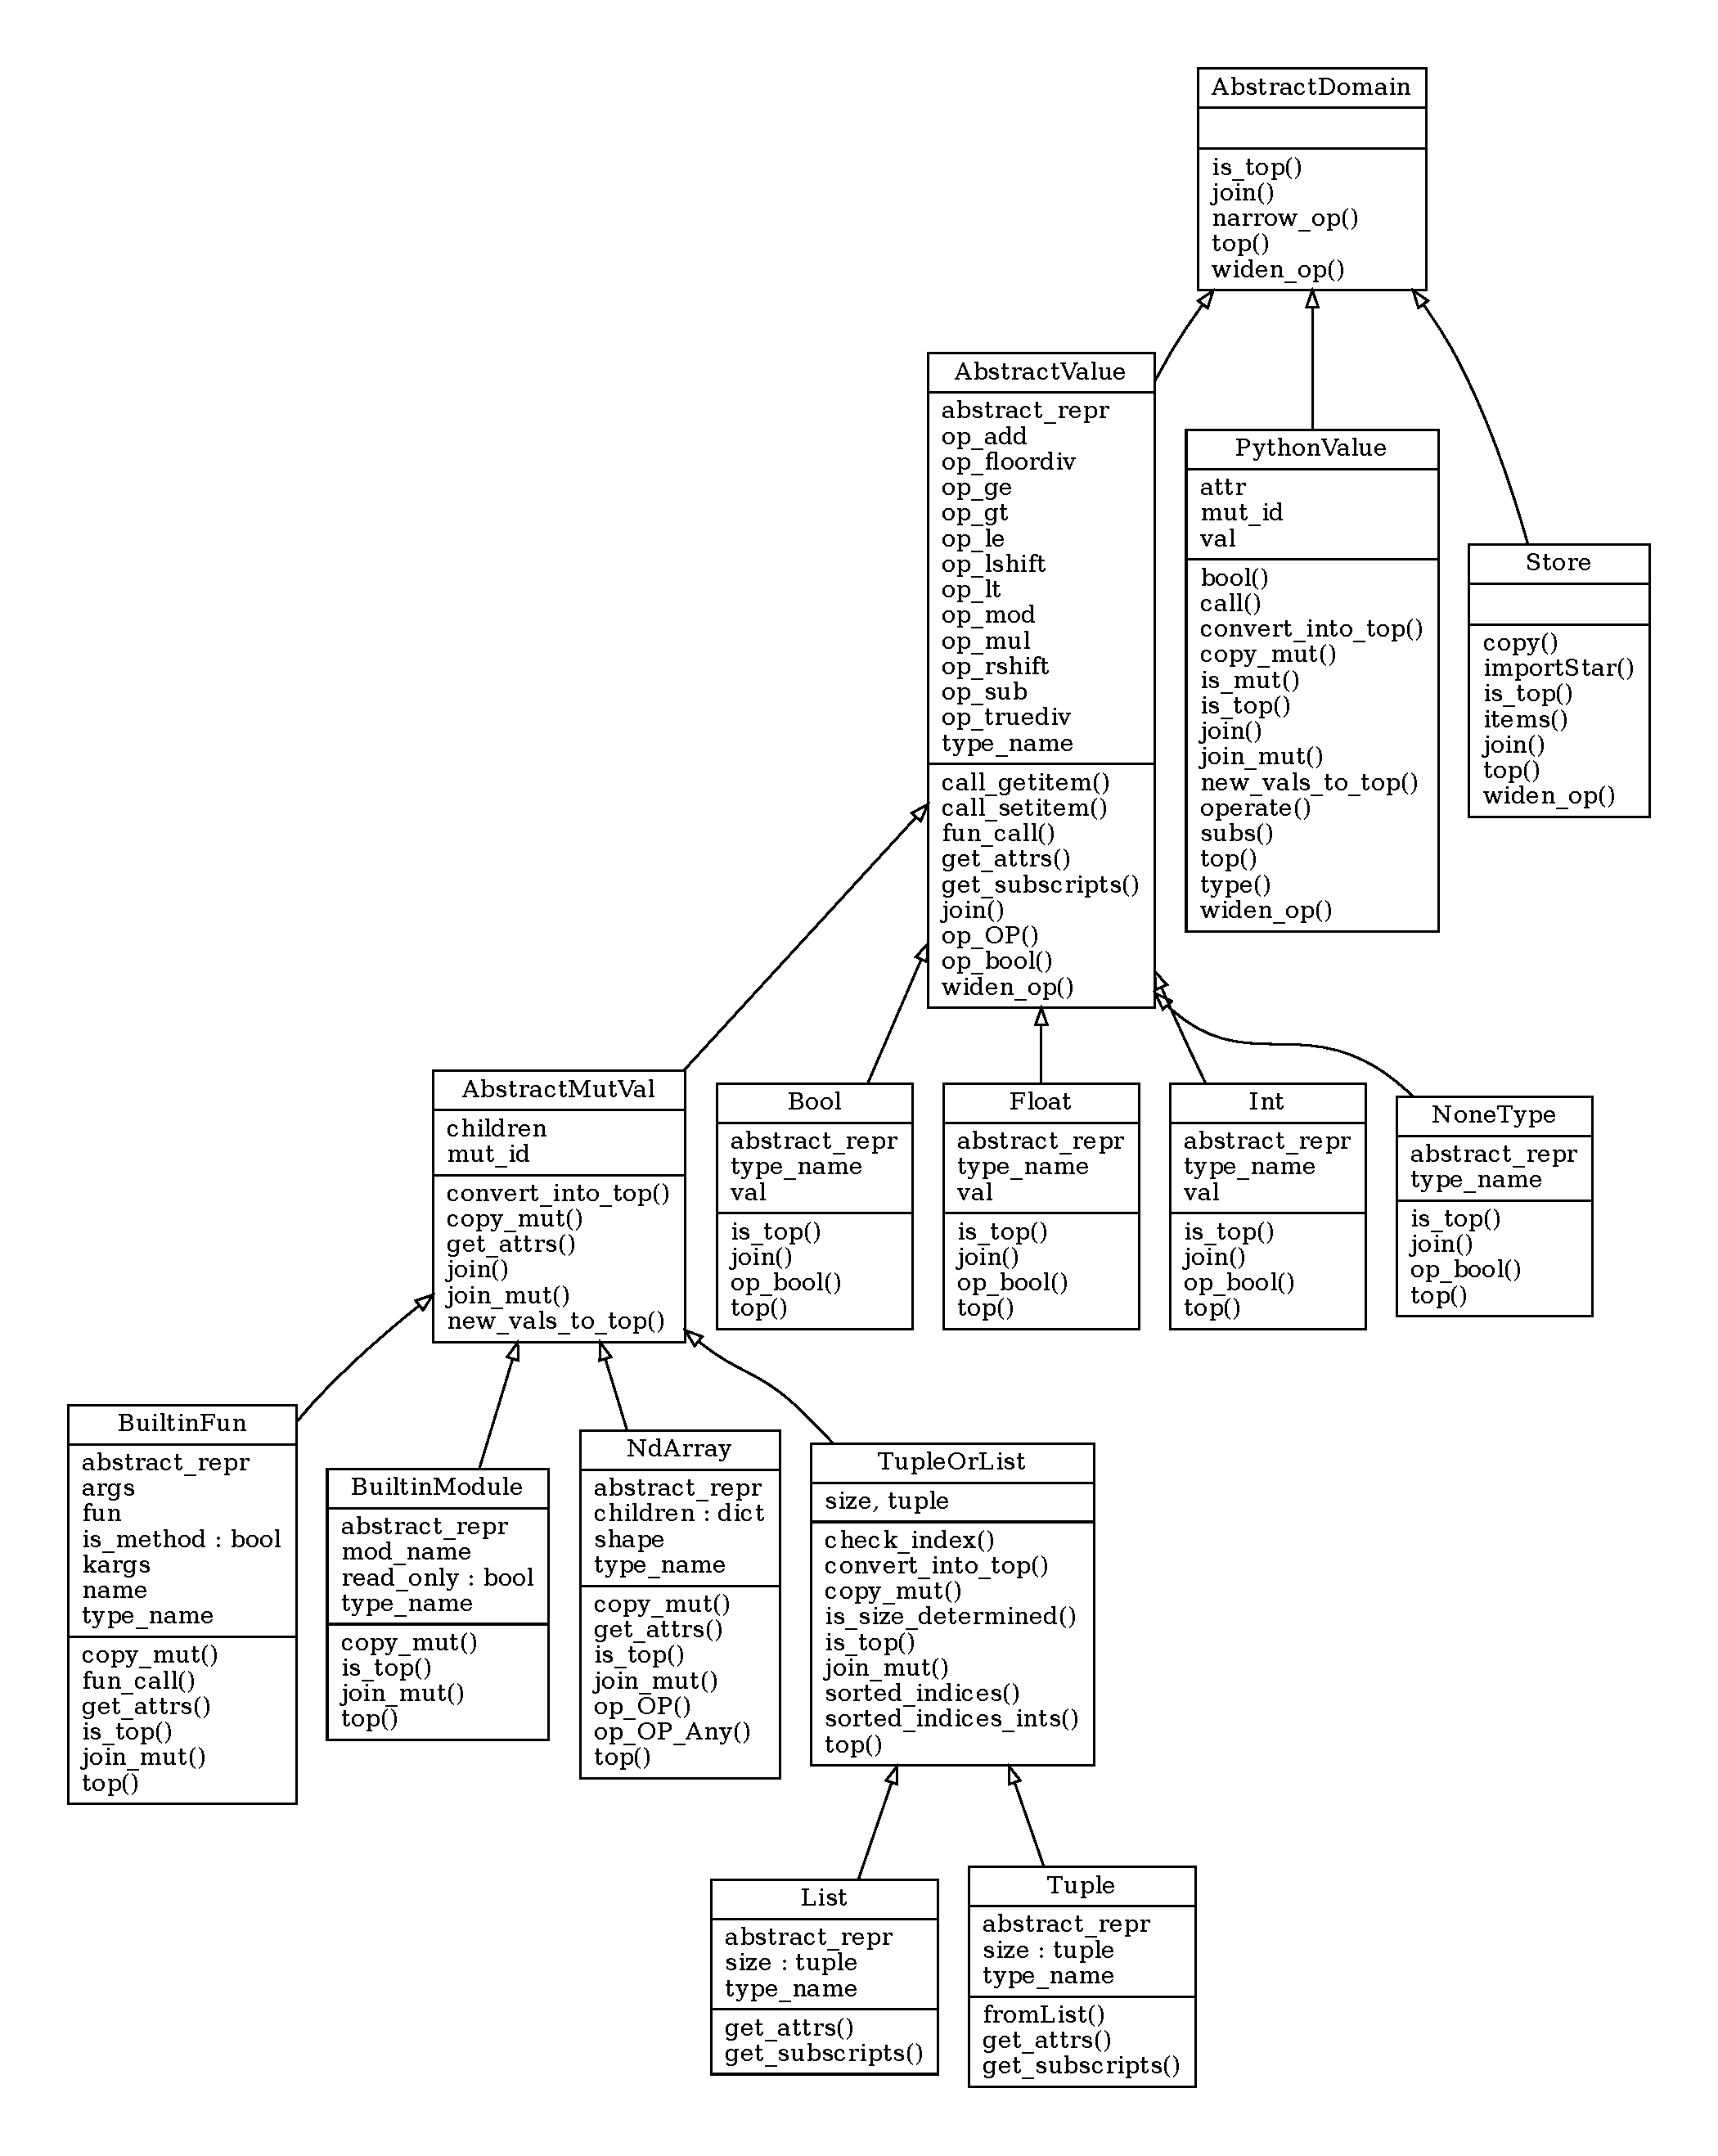
\includegraphics[width=0.95\textwidth]{figures/classes_Pytropos-small.pdf}
\end{center}
\caption{Class diagram for Pytropos, the implementation of the Abstract
  Interpreter.\label{classPytropos}}
\end{figure}

%\todo{add types to each attribute, and add hidden attributes like
%\pycode+__getitem__+}

\texttt{<prim-callable>} and all other \(\mathbf{Object}^\sharp\)s are implemented by a
subclass of \pycode|AbstractMutVal|: \texttt{<prim-callable>} by \pycode|BuiltinFun|,
\texttt{Module} objects by \pycode|BuiltinModule|, \pycode|list|s by \texttt{List}, and
\pycode|tuple| by \texttt{Tuple}.

The implementation of the Abstract Interpreter also includes a class log that stores all
warnings generated in the abstract interpretation of the code.

% \inlinetodo{mention that \texttt{children} is the function \texttt{Key\ -\textgreater{}\
%     Addr\ +\ Undefined}}
% \inlinetodo{mention that \texttt{joinVal} is defined as \texttt{join\_mut} in
%   \texttt{PythonValue}, and \texttt{joinObject} is defined as \texttt{join\_mut} in
%   \texttt{AbstractMutVal}}
